\documentclass[man]{apa6}
\usepackage{lmodern}
\usepackage{amssymb,amsmath}
\usepackage{ifxetex,ifluatex}
\usepackage{fixltx2e} % provides \textsubscript
\ifnum 0\ifxetex 1\fi\ifluatex 1\fi=0 % if pdftex
  \usepackage[T1]{fontenc}
  \usepackage[utf8]{inputenc}
\else % if luatex or xelatex
  \ifxetex
    \usepackage{mathspec}
  \else
    \usepackage{fontspec}
  \fi
  \defaultfontfeatures{Ligatures=TeX,Scale=MatchLowercase}
\fi
% use upquote if available, for straight quotes in verbatim environments
\IfFileExists{upquote.sty}{\usepackage{upquote}}{}
% use microtype if available
\IfFileExists{microtype.sty}{%
\usepackage{microtype}
\UseMicrotypeSet[protrusion]{basicmath} % disable protrusion for tt fonts
}{}
\usepackage{hyperref}
\hypersetup{unicode=true,
            pdftitle={Infants prefer to listen to speech: A meta-analysis.},
            pdfauthor={Cécile Issard, Sho Tsuji, \& Alejandrina Cristia},
            pdfkeywords={Meta-analysis, infants, speech preference, auditory development, natural
sounds},
            pdfborder={0 0 0},
            breaklinks=true}
\urlstyle{same}  % don't use monospace font for urls
\usepackage{graphicx,grffile}
\makeatletter
\def\maxwidth{\ifdim\Gin@nat@width>\linewidth\linewidth\else\Gin@nat@width\fi}
\def\maxheight{\ifdim\Gin@nat@height>\textheight\textheight\else\Gin@nat@height\fi}
\makeatother
% Scale images if necessary, so that they will not overflow the page
% margins by default, and it is still possible to overwrite the defaults
% using explicit options in \includegraphics[width, height, ...]{}
\setkeys{Gin}{width=\maxwidth,height=\maxheight,keepaspectratio}
\IfFileExists{parskip.sty}{%
\usepackage{parskip}
}{% else
\setlength{\parindent}{0pt}
\setlength{\parskip}{6pt plus 2pt minus 1pt}
}
\setlength{\emergencystretch}{3em}  % prevent overfull lines
\providecommand{\tightlist}{%
  \setlength{\itemsep}{0pt}\setlength{\parskip}{0pt}}
\setcounter{secnumdepth}{0}
% Redefines (sub)paragraphs to behave more like sections
\ifx\paragraph\undefined\else
\let\oldparagraph\paragraph
\renewcommand{\paragraph}[1]{\oldparagraph{#1}\mbox{}}
\fi
\ifx\subparagraph\undefined\else
\let\oldsubparagraph\subparagraph
\renewcommand{\subparagraph}[1]{\oldsubparagraph{#1}\mbox{}}
\fi

%%% Use protect on footnotes to avoid problems with footnotes in titles
\let\rmarkdownfootnote\footnote%
\def\footnote{\protect\rmarkdownfootnote}


  \title{Infants prefer to listen to speech: A meta-analysis.}
    \author{Cécile Issard\textsuperscript{1}, Sho Tsuji\textsuperscript{2}, \&
Alejandrina Cristia\textsuperscript{1}}
    \date{}
  
\shorttitle{Preference for speech sounds in infancy}
\affiliation{
\vspace{0.5cm}
\textsuperscript{1} Laboratoire de Sciences Cognitives et Psycholinguistique, Ecole Normale Supérieure, Département d'Études Cognitives\\\textsuperscript{2} University of Tokyo}
\keywords{Meta-analysis, infants, speech preference, auditory development, natural sounds\newline\indent Word count: X}
\usepackage{csquotes}
\usepackage{upgreek}
\captionsetup{font=singlespacing,justification=justified}

\usepackage{longtable}
\usepackage{lscape}
\usepackage{multirow}
\usepackage{tabularx}
\usepackage[flushleft]{threeparttable}
\usepackage{threeparttablex}

\newenvironment{lltable}{\begin{landscape}\begin{center}\begin{ThreePartTable}}{\end{ThreePartTable}\end{center}\end{landscape}}

\makeatletter
\newcommand\LastLTentrywidth{1em}
\newlength\longtablewidth
\setlength{\longtablewidth}{1in}
\newcommand{\getlongtablewidth}{\begingroup \ifcsname LT@\roman{LT@tables}\endcsname \global\longtablewidth=0pt \renewcommand{\LT@entry}[2]{\global\advance\longtablewidth by ##2\relax\gdef\LastLTentrywidth{##2}}\@nameuse{LT@\roman{LT@tables}} \fi \endgroup}


\DeclareDelayedFloatFlavor{ThreePartTable}{table}
\DeclareDelayedFloatFlavor{lltable}{table}
\DeclareDelayedFloatFlavor*{longtable}{table}
\makeatletter
\renewcommand{\efloat@iwrite}[1]{\immediate\expandafter\protected@write\csname efloat@post#1\endcsname{}}
\makeatother
\usepackage{lineno}

\linenumbers

\authornote{

Correspondence concerning this article should be addressed to Cécile
Issard, Laboratoire de Sciences Cognitives et Psycholinguistique, Ecole
Normale Supérieure, Département d'Études Cognitives, 29 rue d'Ulm, 75005
Paris, France. E-mail:
\href{mailto:cecile.issard@gmail.com}{\nolinkurl{cecile.issard@gmail.com}}}

\abstract{
The human auditory system is amazingly efficient at processing speech.
Some works suggest that this capacity is present from birth, infants
preferring to listen to natural speech than to other types of sounds,
enabling them to select the signals that are relevant for communication
with conspecifics. However, in experimental studies, a large variety of
sounds have been contrasted to speech, with infants of very different
ages. Drawing a global picture of how this capacity emerges is therefore
difficult. We synthesized the literature by conducting a meta-analysis
of studies testing speech preference in infants from birth to one year
of age. We found a medium effect size, with infants preferring speech
over any other type of sound. Contrary to the results of individual
studies, we found no effect of age: infants showed the same amount of
preference from birth to one year of age. Still contrary to what
individual studies suggested, we found the same amount of preference
whether speech was contrasted to other natural sounds or to artificial
sounds; as well as whether speech was contrasted to other vocal sounds
or to non-vocal sounds. Preference was stronger when the speech stimuli
were in the infants' native language. This suggests that the
representation of speech as a distinct auditory object comes fromis
modulated by the degree of familiarity with the sounds of the language
they are exposed to.


}

\begin{document}
\maketitle

\begin{itemize}
\tightlist
\item
  Target journal: Developmental science
\item
  Article type: short report
\item
  4000 words
\item
  6 keywords
\item
  Running title: 40 characters
\item
  Submit one normal and one blinded version
\item
  Separate files for title page, main text, and figures
\item
  No identifiying info in the main text.
\item
  up to 4 research highlights; each 25 words
\item
  Abstract: 250 words
\end{itemize}

Main text file:

\begin{enumerate}
\def\labelenumi{\arabic{enumi}.}
\tightlist
\item
  Title
\item
  Research highlights
\item
  Abstract and key words
\item
  Main
\item
  References
\item
  Figures and tables (each clearly identified, labelled and on a
  separate page)
\item
  Appendices (if relevant).
\end{enumerate}

Authors ' contribution: C.I. reviewed literature. C.I. and A.C. coded
data. C.I., S.T. and A.C.analyzed data. C.I. and A.C. wrote the paper.

\section{Introduction}\label{introduction}

Speech is probably the most important sound class for humans. It is the
main signal for vocal communication, and as such it is crucial that
individuals detect this sound in the environment to spot a homospecific
and build social interactions. Readily from birth, humans would be
equipped with a capacity to recognize speech sounds, to process them
with dedicated auditory and cognitive mechanisms. At birth, infants
discriminate speech from complex tones (Dehaene-Lambertz, 2000), and
sine-wave speech (SWS) (Vouloumanos \& Werker, 2007). Extending to
language acquisition, the naturalness of sound stimuli (i.e.~using
synthetic vs.~natural speech) is a key factor for infants to segment
words (Black \& Bergman, 2016). This highlights the importance of
recognizing natural speech sounds in the auditory environment to trigger
the relevant cognitive processes for this stimulus, including for
language acquisition. Discriminating speech from other sounds, and
preferring it over other types of sound, may be a necessary condition to
learn language. Here we synthesize empirical data on infants'
preferences for speech over artificial sounds, natural sounds, as well
as human and social non-speech sounds.

A key question is whether speech is preferred per se, or because it
belongs to a broader category of natural or own-species sounds. Studies
from the auditory neuroscience literature have provided evidence that
natural sounds are processed preferentially by the auditory system, from
the cochlea (Lewicki, 2006) to the auditory cortex (e.g.~Gehr et al.,
2000) (see Mizrahi et al., 2014 for a review). Consistently, infants
have been shown to discriminate between speech and various types of
artificial sounds from birth, from white-noise (Colombo, 1981) to
sine-wave speech (Vouloumanos et al., 2007), low-pass filtered speech
(Cooper, 1994), and backward speech (Peña, 2003; May et al, 2011, 2018).
This preference is maintained to the end of the first year of life
(Curtin, 2013; Vouloumanos, 2014). The infant auditory system would thus
detect general acoustical properties that differentiate artificial from
natural sounds, among them speech. However, studies contrasting speech
to other natural sounds have nuanced this view. Newborns made more
head-turns to speech than to heartbeat (Ecklund-Flores \& Turkewitz,
1996), but listened equivalently to speech and monkey calls (Vouloumanos
\& Werker, 2010). Infants younger than 3 months have been shown to not
discriminate between speech and monkey calls, whereas infants from 3
months of age do (Vouloumanos et al., 2004). It is thus possible that
infants rely on a more specific category for vocal sounds, that includes
our closest genealogical cousins (i.e.~primates), whose vocalizations
may share some important acoustical properties with speech. In an fMRI
study, the activity of the temporal cortex in response to biological
non-speech sounds (such as human non-speech vocalizations or rhesus
calls) decreased with age between 1 and 4 months-old. The response to
speech didn't increase during the same developmental window (Shultz et
al. 2014), suggesting that the capacity to discriminate speech from
other sounds comes from a narrowing of the perceptual category to speech
rather than a more in-depth processing. Infants therefore appear to
discriminate vocal from other natural sounds from the beginning of their
life, and later to discriminate and preferentially process speech
specifically as they get older.

But is it really an effect of age, or does preference come from
familiarity with specific sounds that infants frequently encounter in
their environment? Larger hemodynamic responses were observed in the
newborn brain for forward as compared to backward speech when the native
language was used for the speech stimuli, but not when a foreign
language was used (Sato et al., 2012; May et al., 2018). In 4 month-old
infants, speech produced similar activation patterns for speech and
non-speech vocal sounds, with a larger difference when the speech
stimuli were in the native language of the participants (as compared to
when speech was in a foreign language) (Minagawa-Kawai et al., 2011).
This suggests that infants use their knowledge of the language they are
familiar to to discriminate speech from other sounds. Furthermore, 9
month-old infants listen longer to monkey calls than their native
language (Sorcinelli, 2019), possibly because at this age they are
already attuned to the sounds of their native language and transfer
their attention to the more demanding sound in the paradigm.

Finally, it is possible that the infants' auditory system preferentially
process vocal sounds, and later speech, because they share a complex
acoustical structure. Indeed, studies comparing speech to music often
found a lack of preferential processing. At two months, the temporal
cortex showed the same amount of repetition suppression for speech and
music (Dehaene-Lambertz et al., 2010). Interestingly, this lack of
discrimination persists even after infants discriminate speech from
other complex vocal sounds: at five months, infants detected speech or
music equivalently well in an auditory scene (anonymous, 2019). It is
therefore possible that the developing auditory system is attuned to
complex specific parameters shared by music and speech, but not in other
animal vocalizations.

The complex developmental pattern that we describe above is even more
difficult to understand that controversies exist in the literature. When
speech was compared to other human sounds, two different laboratories
found different patterns: In the first case, speech triggered larger
BOLD responses and looking times than other human sounds, both
communicative (e.g.~laugh or agreement) and non-communicative
(e.g.~yawns or coughs) in 1 to 4 month-old infants (Shultz et al., 2014,
Shultz \& Vouloumanos, 2010). In the second case, the opposite pattern
was observed: human communicative and non-communicative sounds evoked
larger responses than speech in a similar region at 3 months. No
difference between the three types of sounds was observed in the same
infants at 6 months (MacDonald et al., 2019). Moreover, even studies
that found consistent results contrasted speech to a large variety of
sounds, from white noise to filtered speech, and at different ages.
Getting a precise overview of this capacity is therefore difficult. This
points to the importance of synthesizing the available data is a
systematic way.

All of these results have been observed on small groups of infants, with
a large variety of age and stimuli across groups. Individual studies can
only test a few infants on very specific stimuli due to experimental
constraints (Oakes, 2017; Bergmann et al., 2017; Sugden \& Moulson,
2015). On the opposite, meta-analysis are a way of achieving power
without running new studies. They gather data from significantly more
infants than individual studies, which significantly increases
statistical power. By merging a lot of different studies, they allow
researcher to state support (or not) for some results with controversy,
and provide statistical evidence of how much we can trust the results.
If an effect emerges, it's more likely to be a reproducible one that
different labs can find. Finally, meta-analysis offer tools to detect
publication bias in the literature, providing even more evidence to
support or not the results (i.e.~significant effects being less
trustworthy if they emerge from a biased literature). However,
meta-analysis have the disadvantage of mixing studies with different
experimental designs together, therefore having less control on the
effect measured. They merge results focusing on common factors between
studies, potentially missing subtle effects. But moderators analyses
allow to explain the heterogeneity between study. In individual studies,
addressing questions such as differences across stimuli and age groups
types would require large power. Meta-analysis allow to draw a
developmental timeline across the age range covered by the literature,
and test how the different factors discussed by different individual
studies interact. For all of these reasons, we conducted a meta-analysis
to test if infants' reliably have a preference for speech sounds over
other types of sounds, and if yes, if different types of sound modulated
this preference, and how it developed over the first year of life.

\section{Methods}\label{methods}

\subsection{Literature search}\label{literature-search}

We followed PRISMA (Moher et al., 2009). The information sources used to
compose the initial list included suggestions by experts (authors of
this work); two google scholar searches (`` (\enquote{speech preference}
OR \enquote{own-species vocalization} ) AND infant'', and
\enquote{(}speech preference" OR \enquote{own-species vocalization} )
AND infant'') complemented with the same searches in PubMed and
PsycInfo; and a google alert, as well as reference lists of the full
papers inspected. After a first screening based on titles and abstracts,
we ran a second round of screening based on full paper reading.

\subsection{Inclusion criteria}\label{inclusion-criteria}

We included studies that tested human infants from birth to 1 year
(0-365 days) of age, and contrasted speech sounds with any other type of
sound, measuring either behavioral (e.g.~looking times) or
neurophysiological responses to the sounds. We excluded studies that
contrasted foreign to native language, didn't present natural speech
sounds, presented speech recorded with the mother's voice, or
intentionally mixed speech with other vocal sounds within the same sound
condition. We included published (e.i. journal articles) as well as
unpublished works (e.i. doctoral dissertations). A PRISMA flow chart
summarizes the literature review and selection process (Figure 1). We
documented all the studies that we inspected in a decision spreadsheet
(supplementary materials).

{[}Insert Figure 1 here{]}

Data were coded by the first author. 20\% of the papers were selected to
be coded by the second author independently, with disagreements resolved
by discussion. There were \textbf{XX} disagreements out of a total of
\textbf{YY} fields filled in, so that the total agreement rate was
\textbf{ZZ}\%. For effect sizes, we coded the mean score and the
standard deviation for each sound condition. When individual data was
provided, we recomputed the respective mean scores and standard
deviations based on the reported individual scores. When they were
reported, we coded the t-statistic between the two sound conditions or
the F-statistic. If a Cohen's d oran Hedge's g effect size was directly
reported we also coded this. The full list of the variables coded is
available in the supplementary material.

\textbf{Risk assessment at the level of papers was done by \ldots{} Risk
assessment for the whole body of literature \ldots{}}

\subsection{Statistical analysis}\label{statistical-analysis}

\subsubsection{Individual effect sizes}\label{individual-effect-sizes}

Once the data were coded, we computed individual effect sizes that were
not directly reported in the papers, along with their respective
variance. We adjusted the formula according to the experimental design
of the respective paper (Lipsey \& Wilson, 2001). When the coded study
used a within-participant design with two measurements (e.g.~looking
time during speech and during monkey calls), we computed effect size
using t-statistic (Dunlap et al., 1996). If this statistic was not
reported, we computed effect size based on the respective means and SDs.
We then corrected the computed effect size with the correlation between
the two measurements. We computed this correlation based on the
t-statistic, the respective means and SDs (Lipsey \& Wilson, 2001). If
not all of these informations were reported, we randomly imputed a
correlation with equal probability between 0.01 and 0.99.

Effect sizes were first computed as Cohen's d, and then transformed to
Hedge's g.

\subsubsection{Meta-analytic models}\label{meta-analytic-models}

Once the data was completed, we estimated the true effect size fitting
mixed-effects meta-analytic regressions. We used the R package metafor
\textbf{(CITE)}. We specified a hierarchical model with random effects
of paper, and random effects for independent infants within paper
(same\_infant). We specified the following moderators as fixed effects:
- mean age of children; - experimental method (Central
fixation/Head-turn Preference Procedure/High Amplitude Sucking/Passive
Listening); - familiarity with the language used (native/foreign); -
naturalness of the contrastive sound (natural/artificial, coded as
yes/no). If the sound contrasted to speech was natural, we also coded
whether it was vocal or not, and from human or another species
(homospecific/heterospecific, coded as yes/no).

We first estimated the global effect size by fitting a random-effects
meta-analytic regression without any hierarchical structure or
moderator. We then added the hierarchical structure with papers and
infant groups within papers. We assessed whether the experimental method
influenced the magnitude of the effect size apart from target moderators
by fitting a mixed-effects meta-analytic regression with the above
described hierarchical structure and the method as a moderator.

We investigated the effect of familiarity with the sound by running a
mixed-effects meta-analytic model with nativeness of the language used
for the speech stimuli as a moderator.

We then investigated whether speech preference was embedded in a
preference for natural sounds, and whether this potential effect evolved
over the course of the first year of life, by fitting a mixed-effects
meta-analytic model with naturalness and age as moderators. To
facilitate result interpretation, we centered age.

Finally, we subsetted the dataset to contrasts between speech and
natural sounds, and fitted a meta-analytic regression on this subset
with vocalness (vocal/non-vocal), and species
(homospecific/heterospecific) as moderators.

\begin{verbatim}
##          
##           no yes
##   foreign 12  32
##   native  29   8
\end{verbatim}

\begin{verbatim}
## RVE: Hierarchical Effects Model with Small-Sample Corrections 
## 
## Model: g_calc ~ test_lang * mean_age_1 + natural * mean_age_1 + vocal * mean_age_1 + method 
## 
## Number of clusters = 39 
## Number of outcomes = 81 (min = 1 , mean = 2.08 , median = 2 , max = 8 )
## Omega.sq = 0.1044145 
## Tau.sq = 0.09461373 
## 
##                           Estimate  StdErr t-value  dfs P(|t|>) 95% CI.L
## 1           X.Intercept.  0.798650 0.30110   2.652 8.46 0.02777  0.11088
## 2             test_lang2  0.021449 0.18339   0.117 6.81 0.91027 -0.41466
## 3             mean_age_1 -0.001286 0.00225  -0.571 4.25 0.59674 -0.00740
## 4               natural1 -0.059219 0.19144  -0.309 4.27 0.77159 -0.57793
## 5                 vocal1 -0.020689 0.19132  -0.108 4.19 0.91887 -0.54274
## 6                method2 -0.747835 0.29426  -2.541 2.28 0.11075 -1.87436
## 7                method3 -0.181230 0.27496  -0.659 8.89 0.52653 -0.80445
## 8                method4 -0.532540 0.15288  -3.483 9.47 0.00638 -0.87576
## 9  test_lang2.mean_age_1  0.000808 0.00120   0.670 8.07 0.52130 -0.00197
## 10   mean_age_1.natural1  0.001906 0.00151   1.264 6.63 0.24888 -0.00170
## 11     mean_age_1.vocal1 -0.002116 0.00194  -1.088 7.12 0.31192 -0.00670
##    95% CI.U Sig
## 1   1.48642  **
## 2   0.45756    
## 3   0.00482    
## 4   0.45949    
## 5   0.50137    
## 6   0.37869    
## 7   0.44199    
## 8  -0.18932 ***
## 9   0.00358    
## 10  0.00551    
## 11  0.00247    
## ---
## Signif. codes: < .01 *** < .05 ** < .10 *
## ---
## Note: If df < 4, do not trust the results
\end{verbatim}

\begin{verbatim}
## RVE: Hierarchical Effects Model with Small-Sample Corrections 
## 
## Model: g_calc ~ test_lang + natural * mean_age_1 
## 
## Number of clusters = 39 
## Number of outcomes = 81 (min = 1 , mean = 2.08 , median = 2 , max = 8 )
## Omega.sq = 0.08187635 
## Tau.sq = 0.1160369 
## 
##                        Estimate  StdErr t-value   dfs P(|t|>) 95% CI.L
## 1        X.Intercept.  0.304513 0.20052  1.5186  7.03   0.172 -0.16918
## 2          test_lang2  0.164845 0.11567  1.4251 13.86   0.176 -0.08348
## 3            natural1 -0.134247 0.20704 -0.6484 10.04   0.531 -0.59532
## 4          mean_age_1  0.000126 0.00206  0.0611  6.50   0.953 -0.00482
## 5 natural1.mean_age_1  0.000497 0.00215  0.2313 10.00   0.822 -0.00429
##   95% CI.U Sig
## 1  0.77821    
## 2  0.41317    
## 3  0.32682    
## 4  0.00507    
## 5  0.00528    
## ---
## Signif. codes: < .01 *** < .05 ** < .10 *
## ---
## Note: If df < 4, do not trust the results
\end{verbatim}

\begin{verbatim}
## RVE: Hierarchical Effects Model with Small-Sample Corrections 
## 
## Model: g_calc ~ test_lang + vocal * mean_age_1 
## 
## Number of clusters = 39 
## Number of outcomes = 81 (min = 1 , mean = 2.08 , median = 2 , max = 8 )
## Omega.sq = 0.07825038 
## Tau.sq = 0.1175162 
## 
##                      Estimate  StdErr t-value   dfs P(|t|>) 95% CI.L
## 1      X.Intercept.  0.374847 0.18869   1.987  9.82  0.0756 -0.04664
## 2        test_lang2  0.128812 0.11787   1.093 21.60  0.2865 -0.11590
## 3            vocal1 -0.224538 0.18456  -1.217 15.01  0.2425 -0.61788
## 4        mean_age_1 -0.000268 0.00211  -0.127  7.49  0.9023 -0.00519
## 5 vocal1.mean_age_1  0.001117 0.00220   0.509 11.75  0.6203 -0.00368
##   95% CI.U Sig
## 1  0.79633   *
## 2  0.37352    
## 3  0.16881    
## 4  0.00465    
## 5  0.00591    
## ---
## Signif. codes: < .01 *** < .05 ** < .10 *
## ---
## Note: If df < 4, do not trust the results
\end{verbatim}

\begin{verbatim}
## 
##        animal      backward    BPfiltered       com_voc complex_tones 
##             1            22             2             7             1 
##    duck_calls      emotions environmental     heartbeat   heartspeech 
##             2             2             3             2             2 
##    HPfiltered human_walking    LPfiltered  monkey_calls         music 
##             2             1             5            11             3 
##   non-com_voc     scrambled           SWS         water   white_noise 
##             7             2            10             4             2
\end{verbatim}

\begin{verbatim}
##        animal      backward    BPfiltered       com_voc complex_tones 
##    1.07499753    0.33642725    0.37521239    0.12226565           NaN 
##    duck_calls      emotions environmental     heartbeat   heartspeech 
##    1.26795256   -0.16579236    0.27993843    1.02131722    1.43229167 
##    HPfiltered human_walking    LPfiltered  monkey_calls         music 
##    0.83689393    0.48158905    1.23310038    0.42686707   -0.30122164 
##   non-com_voc     scrambled           SWS         water   white_noise 
##    0.38626556    0.02319572    0.33526236    0.36152402    1.08797229
\end{verbatim}

\begin{verbatim}
## 
## Multivariate Meta-Analysis Model (k = 81; method: REML)
## 
##    logLik   Deviance        AIC        BIC       AICc  
## -127.2568   254.5137   262.5137   271.9915   263.0542  
## 
## Variance Components: 
## 
##             estim    sqrt  nlvls  fixed                factor
## sigma^2.1  0.0287  0.1695     24     no              study_ID
## sigma^2.2  0.0794  0.2818     39     no  study_ID/same_infant
## 
## Test for Residual Heterogeneity: 
## QE(df = 79) = 450.7595, p-val < .0001
## 
## Test of Moderators (coefficient(s) 2): 
## QM(df = 1) = 3.1427, p-val = 0.0763
## 
## Model Results:
## 
##             estimate      se    zval    pval    ci.lb   ci.ub    
## intrcpt       0.2527  0.0810  3.1195  0.0018   0.0939  0.4115  **
## test_lang2    0.1576  0.0889  1.7728  0.0763  -0.0166  0.3319   .
## 
## ---
## Signif. codes:  0 '***' 0.001 '**' 0.01 '*' 0.05 '.' 0.1 ' ' 1
\end{verbatim}

\begin{verbatim}
## 
## Multivariate Meta-Analysis Model (k = 81; method: REML)
## 
##    logLik   Deviance        AIC        BIC       AICc  
## -128.2582   256.5164   264.5164   273.9942   265.0570  
## 
## Variance Components: 
## 
##             estim    sqrt  nlvls  fixed                factor
## sigma^2.1  0.0180  0.1342     24     no              study_ID
## sigma^2.2  0.0880  0.2966     39     no  study_ID/same_infant
## 
## Test for Residual Heterogeneity: 
## QE(df = 79) = 451.5476, p-val < .0001
## 
## Test of Moderators (coefficient(s) 2): 
## QM(df = 1) = 1.1710, p-val = 0.2792
## 
## Model Results:
## 
##          estimate      se     zval    pval    ci.lb   ci.ub     
## intrcpt    0.4022  0.0838   4.8008  <.0001   0.2380  0.5663  ***
## vocal1    -0.0983  0.0909  -1.0821  0.2792  -0.2765  0.0798     
## 
## ---
## Signif. codes:  0 '***' 0.001 '**' 0.01 '*' 0.05 '.' 0.1 ' ' 1
\end{verbatim}

\subsubsection{Publication bias}\label{publication-bias}

We assessed the presence of a potential publication bias in the
literature by plotting N funnel plots. The first one was based on the
simple model without hierarchical structure nor moderators. We
symmetrized this funnel plot using the \enquote{trim and fill} method
(ADD REF). The second funnel plot was based on the mixed model with
hierarchical random structure and moderators. We tested the asymmetry of
the funnel plots by regressing effect size as a function of effect size
standard error and running a Kendall's tau rank test.

\section{Results}\label{results}

\subsection{Database description}\label{database-description}

We found a total of 29 papers reporting 98 (not mutually independent)
effect sizes, see Table 1. All of them have been submitted to or
published in peer-reviewed journals. Studies tended to have small sample
sizes, with a median N of 20 children (Range = 55, M = 21.39, Total:
963). Infants ranged from 0 to 12 months (1.21 to 380.50 days).
Individual samples comprised 20 \% of female participants on average.
Infants were native of 7 different languages across the whole database
(English, French, Japanese, Italian, Russian, Yiddish, Hebrew). Studies
were performed in 13 different laboratories from 6 different countries
(United States, Canada, Israel, France, Japan, Italy). 4 experimental
methods were used: 11 studies used Passive Listening (PL) with
neuro-imaging, with 8 studies using Near-Infrared Spectroscopy (NIRS),
and 3 studies using fMRI; 12 studies used Central Fixation (CF); 3 used
High-Amplitude Sucking (HAS); and 1 used Head-turn Preference Procedure
(HPP).

\begin{verbatim}
## 
## 
## \begin{table}[tbp]
## \begin{center}
## \begin{threeparttable}
## \caption{\label{tab:DB_summary}Variables of interest for each individual study}
## \begin{tabular}{lllllllll}
## \toprule
## short\_cite & \multicolumn{1}{c}{g\_calc} & \multicolumn{1}{c}{g\_var\_calc} & \multicolumn{1}{c}{method} & \multicolumn{1}{c}{n\_1} & \multicolumn{1}{c}{mean\_age\_1} & \multicolumn{1}{c}{test\_lang} & \multicolumn{1}{c}{vocal} & \multicolumn{1}{c}{natural}\\
## \midrule
## May et al. (2018) & 0.83 & 0.04 & PL & 20 & 1.21 & foreign & no & no\\
## May et al. (2018) & 0.35 & 0.04 & PL & 20 & 1.21 & foreign & no & no\\
## May et al. (2018) & 0.14 & 0.03 & PL & 20 & 1.21 & foreign & no & no\\
## May et al. (2018) & -0.08 & 0.03 & PL & 20 & 1.21 & foreign & no & no\\
## May et al. (2018) & 0.57 & 0.04 & PL & 24 & 1.46 & native & no & no\\
## May et al. (2018) & 0.33 & 0.08 & PL & 24 & 1.46 & native & no & no\\
## May et al. (2018) & 0.07 & 0.03 & PL & 24 & 1.46 & foreign & no & no\\
## May et al. (2018) & -0.01 & 0.02 & PL & 24 & 1.46 & foreign & no & no\\
## Ecklund-Flores \& Turkewitz (1996) & -0.57 & 0.15 & HPP & 12 & 1.50 & native & no & yes\\
## Ecklund-Flores \& Turkewitz (1996) & 2.62 & 0.37 & HPP & 12 & 1.50 & native & no & yes\\
## Ecklund-Flores \& Turkewitz (1996) & 0.00 & 0.04 & HPP & 12 & 1.50 & native & yes & yes\\
## Ecklund-Flores \& Turkewitz (1996) & 0.87 & 0.07 & HPP & 12 & 1.50 & native & yes & yes\\
## Ecklund-Flores \& Turkewitz (1996) & 0.11 & 0.09 & HPP & 10 & 1.50 & native & yes & no\\
## Ecklund-Flores \& Turkewitz (1996) & 1.57 & 0.18 & HPP & 10 & 1.50 & native & yes & no\\
## Ecklund-Flores \& Turkewitz (1996) & 0.13 & 0.05 & HPP & 14 & 1.50 & native & yes & no\\
## Ecklund-Flores \& Turkewitz (1996) & 0.62 & 0.14 & HPP & 14 & 1.50 & native & yes & no\\
## Ecklund-Flores \& Turkewitz (1996) & 0.23 & 0.07 & HPP & 11 & 1.50 & native & yes & no\\
## Ecklund-Flores \& Turkewitz (1996) & 2.64 & 0.36 & HPP & 11 & 1.50 & native & yes & no\\
## May et al. (2011) & 0.01 & 0.04 & PL & 20 & 1.60 & native & no & no\\
## May et al. (2011) & -0.05 & 0.02 & PL & 20 & 1.60 & native & no & no\\
## May et al. (2011) & -0.15 & 0.09 & PL & 20 & 1.60 & foreign & no & no\\
## May et al. (2011) & -0.10 & 0.05 & PL & 20 & 1.60 & foreign & no & no\\
## Vouloumanos \& Werker (2007) & 0.50 & 0.04 & HAS & 22 & 1.88 & native & no & no\\
## Vouloumanos \& Werker (2007) & -0.26 & 0.05 & HAS & 22 & 1.88 & native & no & no\\
## Vouloumanos et al. (2010) & -0.19 & 0.03 & HAS & 30 & 1.96 & native & yes & yes\\
## Cristia et al. (2014) & -0.09 & 0.02 & PL & 31 & 2.00 & foreign & yes & yes\\
## Cristia et al. (2014) & -0.24 & 0.02 & PL & 30 & 2.00 & foreign & yes & yes\\
## Cristia et al. (2014) & NA & NA & PL & 28 & 2.00 & NA & NA & NA\\
## Cristia et al. (2014) & NA & NA & PL & 28 & 2.00 & NA & NA & NA\\
## Cristia et al. (2014) & NA & NA & PL & 30 & 2.00 & NA & NA & NA\\
## Spence \& DeCasper (1987) & NA & NA & HAS & 8 & 2.00 & native & yes & yes\\
## Bartha-Doering et al. (2019) & 0.98 & 0.10 & PL & 15 & 2.17 & native & no & no\\
## Bartha-Doering et al. (2019) & 0.30 & 0.03 & PL & 15 & 2.17 & native & no & no\\
## Pena et al. (2003) & 0.85 & 0.11 & PL & 12 & 2.70 & native & no & no\\
## Pena et al. (2003) & 0.71 & 0.06 & PL & 12 & 2.70 & native & no & no\\
## Sato et al. (2012) & NA & NA & PL & 17 & 4.40 & NA & no & no\\
## Sato et al. (2012) & NA & NA & PL & 17 & 4.40 & NA & no & no\\
## Sato et al. (2012) & NA & NA & PL & 17 & 4.40 & NA & no & no\\
## Sato et al. (2012) & NA & NA & PL & 17 & 4.40 & NA & no & no\\
## Cooper \& Aslin (1994) & 0.55 & 0.07 & CF & 16 & 34.00 & native & yes & no\\
## Dehaene-Lambertz (2000) & NA & NA & PL & 15 & 116.00 & native & no & no\\
## Dehaene-Lambertz et al. (2010) & -0.33 & 0.06 & PL & 7 & 72.00 & native & no & no\\
## Dehaene-Lambertz et al. (2010) & -0.06 & 0.06 & PL & 7 & 72.00 & native & no & no\\
## Vouloumanos \& Werker (2004) & 0.35 & 0.03 & CF & 16 & 76.88 & native & no & no\\
## Shultz et al. (2014) & NA & NA & PL & 24 & 78.00 & foreign & NA & NA\\
## Shultz et al. (2014) & 0.44 & 0.02 & PL & 24 & 78.00 & foreign & yes & yes\\
## Shultz et al. (2014) & 0.48 & 0.06 & PL & 24 & 78.00 & foreign & no & yes\\
## Shultz et al. (2014) & 0.28 & 0.02 & PL & 24 & 78.00 & foreign & yes & yes\\
## Shultz et al. (2014) & 0.31 & 0.03 & PL & 24 & 78.00 & foreign & yes & yes\\
## Dehaene-Lambertz et al. (2002) & NA & NA & PL & 20 & 79.00 & native & no & no\\
## Mc Donald et al. (2019) & -0.65 & 0.04 & PL & 35 & 94.53 & foreign & yes & yes\\
## Mc Donald et al. (2019) & 1.71 & 0.05 & PL & 35 & 94.53 & foreign & yes & yes\\
## Mc Donald et al. (2019) & -0.86 & 0.04 & PL & 35 & 94.53 & foreign & yes & yes\\
## Mc Donald et al. (2019) & 1.30 & 0.05 & PL & 35 & 94.53 & foreign & yes & yes\\
## Vouloumanos et al. (2010) & 1.59 & 0.11 & CF & 16 & 100.00 & native & yes & yes\\
## Shultz \& Vouloumanos (2010) & NA & NA & CF & 23 & 102.00 & foreign & NA & NA\\
## Shultz \& Vouloumanos (2010) & 0.52 & 0.04 & CF & 23 & 102.00 & foreign & yes & yes\\
## Shultz \& Vouloumanos (2010) & 0.45 & 0.04 & CF & 23 & 102.00 & foreign & yes & yes\\
## Shultz \& Vouloumanos (2010) & 0.27 & 0.05 & CF & 23 & 102.00 & foreign & no & yes\\
## Shultz \& Vouloumanos (2010) & NA & NA & CF & 23 & 102.00 & foreign & NA & NA\\
## Shultz \& Vouloumanos (2010) & NA & NA & CF & 14 & 111.00 & foreign & NA & NA\\
## Shultz \& Vouloumanos (2010) & 0.63 & 0.07 & CF & 14 & 111.00 & foreign & yes & yes\\
## Shultz \& Vouloumanos (2010) & 0.62 & 0.06 & CF & 14 & 111.00 & foreign & yes & yes\\
## Shultz \& Vouloumanos (2010) & 0.22 & 0.01 & CF & 48 & 116.00 & foreign & no & yes\\
## Shultz \& Vouloumanos (2010) & 0.56 & 0.08 & CF & 25 & 116.00 & foreign & no & yes\\
## Shultz \& Vouloumanos (2010) & 0.43 & 0.02 & CF & 25 & 116.00 & foreign & no & yes\\
## Shultz \& Vouloumanos (2010) & 0.36 & 0.02 & CF & 25 & 116.00 & foreign & no & yes\\
## Minagawa-Kawai et al. (2011) & 0.07 & 0.04 & PL & 12 & 128.00 & native & yes & yes\\
## Minagawa-Kawai et al. (2011) & -0.06 & 0.08 & PL & 12 & 128.00 & foreign & yes & yes\\
## Minagawa-Kawai et al. (2011) & 0.09 & 0.04 & PL & 12 & 128.00 & native & no & no\\
## Minagawa-Kawai et al. (2011) & -0.04 & 0.05 & PL & 12 & 128.00 & foreign & no & no\\
## Colombo \& Bundy (1981) & 0.47 & 0.04 & CF & 14 & 131.00 & native & no & no\\
## Vouloumanos \& Werker (2004) & 0.47 & 0.05 & CF & 16 & 140.76 & native & no & no\\
## Vouloumanos et al. (2009) & NA & NA & CF & 15 & 151.76 & foreign & yes & yes\\
## Vouloumanos et al. (2009) & NA & NA & CF & 12 & 152.20 & foreign & yes & yes\\
## Vouloumanos et al. (2009) & 0.56 & 0.07 & CF & 12 & 152.20 & foreign & yes & yes\\
## Vouloumanos et al. (2009) & 1.05 & 0.09 & CF & 12 & 156.20 & foreign & yes & yes\\
## Vouloumanos et al. (2009) & 1.31 & 0.11 & CF & 12 & 156.20 & foreign & yes & yes\\
## Vouloumanos et al. (2009) & 1.23 & 0.08 & CF & 15 & 157.20 & foreign & yes & yes\\
## Vouloumanos et al. (2009) & 0.89 & 0.08 & CF & 15 & 157.20 & foreign & yes & yes\\
## anonymous (2019) & -0.51 & 0.04 & CF & 30 & 159.20 & native & no & no\\
## anonymous (2019) & 0.25 & 0.03 & CF & 30 & 159.20 & native & no & yes\\
## anonymous (2019) & 0.20 & 0.04 & CF & 19 & 164.20 & foreign & no & yes\\
## anonymous (2019) & 1.07 & 0.07 & CF & 19 & 164.20 & foreign & yes & yes\\
## Mc Donald et al. (2019) & 0.43 & 0.04 & PL & 35 & 187.05 & foreign & yes & yes\\
## Mc Donald et al. (2019) & -0.24 & 0.02 & PL & 35 & 187.05 & foreign & yes & yes\\
## Mc Donald et al. (2019) & -0.22 & 0.01 & PL & 35 & 187.05 & foreign & yes & yes\\
## Mc Donald et al. (2019) & -0.98 & 0.04 & PL & 35 & 187.05 & foreign & yes & yes\\
## Vouloumanos \& Werker (2004) & 0.42 & 0.03 & CF & 16 & 196.64 & foreign & no & no\\
## Sorcinelli et al. (2019) & 0.25 & 0.01 & CF & 60 & 277.00 & foreign & no & no\\
## Yamashiro et al. (2019) & 0.45 & 0.03 & CF & 34 & 277.00 & foreign & no & no\\
## Sorcinelli et al. (2019) & -0.23 & 0.01 & CF & 54 & 280.05 & foreign & yes & yes\\
## Segal \& Kishon-Rabin (2011) & 1.71 & 0.15 & CF & 22 & 308.05 & native & no & no\\
## Segal \& Kishon-Rabin (2011) & 0.98 & 0.07 & CF & 21 & 308.05 & native & no & no\\
## Curtin \& Vouloumanos (2013) & 0.46 & 0.05 & CF & 28 & 379.59 & native & no & no\\
## Vouloumanos \& Curtin (2014) & 0.51 & 0.05 & CF & 27 & 380.50 & native & no & no\\
## Ference (2018) & 0.20 & 0.01 & CF & 58 & 182.64 & native & no & no\\
## Sambeth et al. (2008) & 3.52 & 1.30 & PL & 5 & 2.00 & native & yes & yes\\
## \bottomrule
## \end{tabular}
## \end{threeparttable}
## \end{center}
## \end{table}
\end{verbatim}

\subsection{Summary effect size}\label{summary-effect-size}

We found a mean weighted effect size g = (SE = CI{[},{]}).

\begin{verbatim}
## pdf 
##   2
\end{verbatim}

\subsection{Publication bias}\label{publication-bias-1}

Evidence of bias at level of papers Evidence of bias at level of
literature

\begin{figure}

{\centering 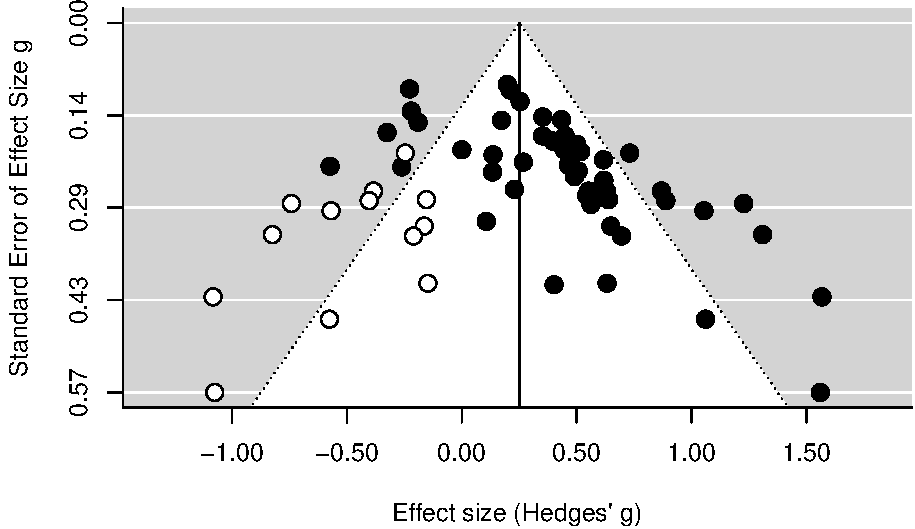
\includegraphics{MA_speech_pref_files/figure-latex/publication bias-1} 

}

\caption{ }(\#fig:publication bias)
\end{figure}

\begin{verbatim}
## 
## Regression Test for Funnel Plot Asymmetry
## 
## model:     mixed-effects meta-regression model
## predictor: standard error
## 
## test for funnel plot asymmetry: z = 6.8548, p < .0001
\end{verbatim}

\begin{verbatim}
## 
## Rank Correlation Test for Funnel Plot Asymmetry
## 
## Kendall's tau = 0.3550, p < .0001
\end{verbatim}

\subsection{Main effects}\label{main-effects}

\begin{verbatim}
##      CF     HAS     HPP      PL 
## "black"  "blue"   "red" "green"
\end{verbatim}

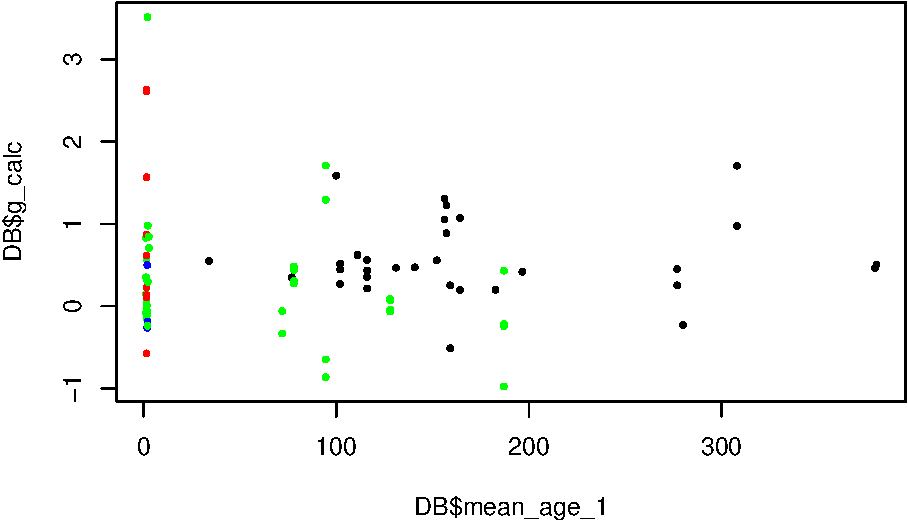
\includegraphics{MA_speech_pref_files/figure-latex/plots-1.pdf}
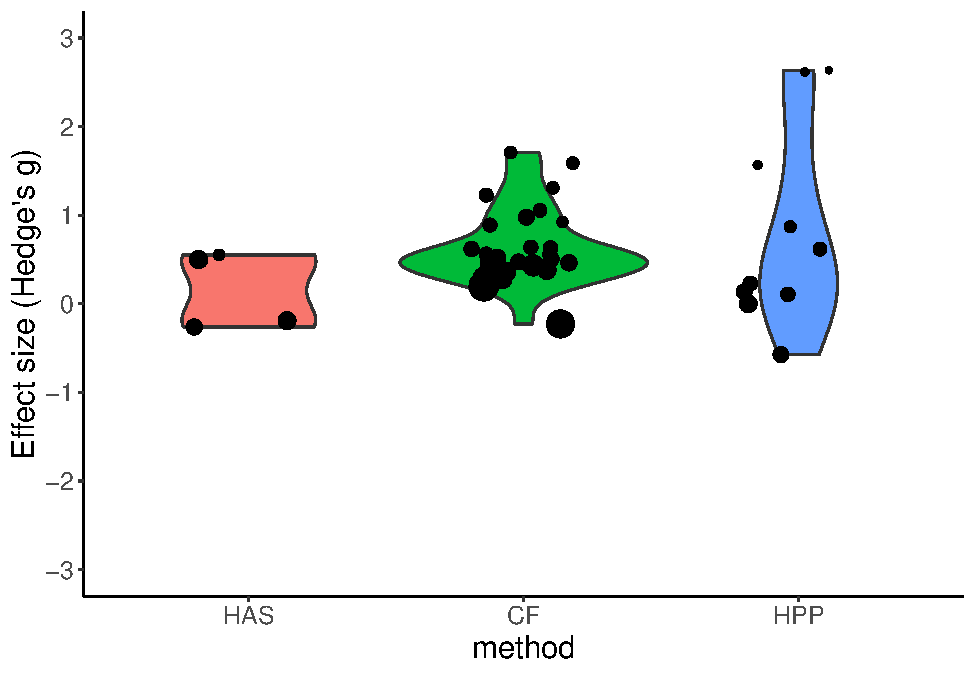
\includegraphics{MA_speech_pref_files/figure-latex/plots-2.pdf}
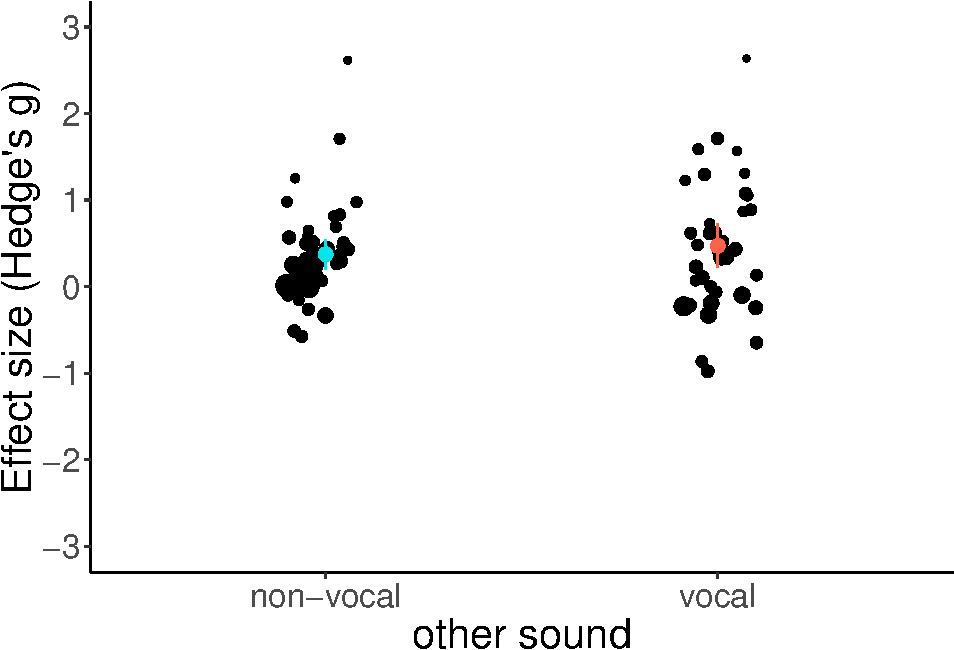
\includegraphics{MA_speech_pref_files/figure-latex/plots-3.pdf}
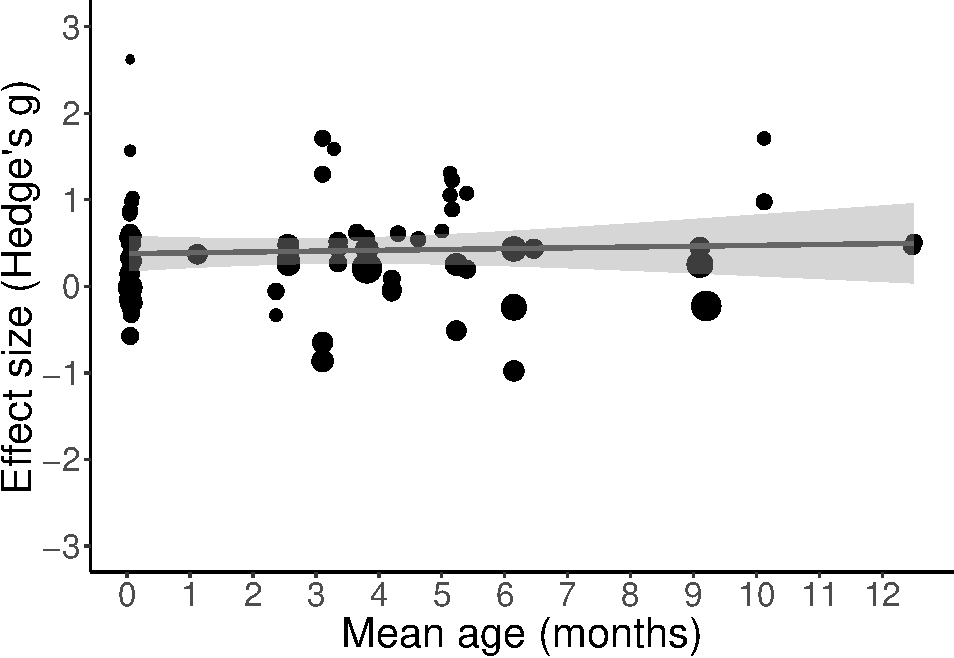
\includegraphics{MA_speech_pref_files/figure-latex/plots-4.pdf}
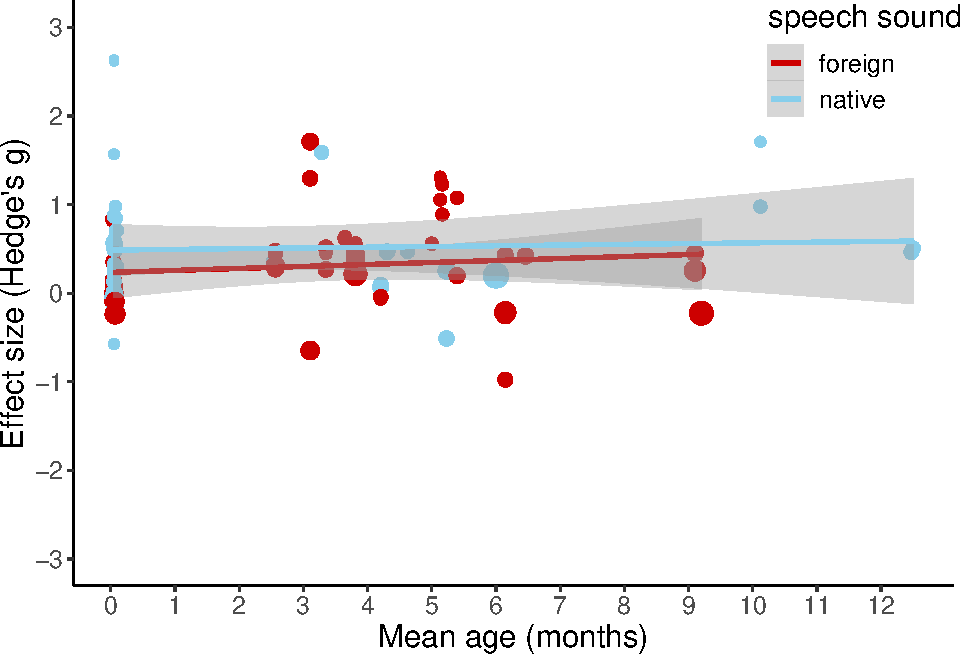
\includegraphics{MA_speech_pref_files/figure-latex/plots-5.pdf}

Heterogeneity Moderators age, type \& interaction

\section{Discussion}\label{discussion}

\begin{itemize}
\tightlist
\item
  Age
\item
  Type of sounds contrasted
\item
  Interactions
\item
  power
\item
  heterogeneity
\end{itemize}

Naturalness alone doesn't significantly moderate infants' preference for
speech sounds: they still prefer speech, and the amount of preference
doesn't change, whether the sound is natural or artificial. This means
that infants prefer natural speech in itself. This preference might
explain why naturalness makes a difference for higher-level linguistic,
a priori abstract tasks such as word segmentation (Black \& Bergmann,
2016): speech triggers different cognitive mechanisms than other sounds.
Not incompatible as in this meta-analysis natural speech stimuli when
contrasted to only synthetic speech. We don't know if infants would have
been able to find \enquote{words} with natural sounds other than
syllables (i.e.~frequent sequences of several natural sounds).

{[}Significant effect of the language used for speech sounds:
familiarity with the sound patterns of the infants' native language
amplifies the preference for speech sounds. -\textgreater{} Contribution
of perceptual learning.{]}NATIVE \& FOREIGN HAVE CLOSE DISTRIBUTIONS
(SEE VIOLIN PLOT), ONLY SIG. FOR MODELS FITTED WITH METAFOR!!!

Preferential processing of speech may support higher level cognitive
tasks, such as categorization (Waxman, 1997; 2007; 2010).

Experimental method significantly modulates speech preference: some
methods are more appropriate than others to test infants on this type of
task. This phenomenon has been repeatedly observed in developmental
meta-analysis (see Bergmann et al., 2018, for a synthesis across
meta-analysis in developmental psychology).

Necessity to : - test infants between 9 and 12 months old on natural
vocal stimuli. - test preference against music. - test infants between 9
and 12 months old using a foreign language.

\newpage

\begingroup
\setlength{\parindent}{-0.5in} \setlength{\leftskip}{0.5in}

\hypertarget{refs}{}

\endgroup


\end{document}
